\documentclass[10pt,a4paper,twocolumn,DIV18]{scrartcl}   

\PassOptionsToPackage{hyphens}{url}\usepackage[linktocpage,bookmarks]{hyperref}
\hypersetup{    pdfauthor={Name des Authors},
                pdftitle={Titel},
                pdfsubject={},
                colorlinks=true,
                citecolor=black,
                linkcolor=black,
                urlcolor=black}
\usepackage[latin1]{inputenc}
\usepackage[T1]{fontenc}
\usepackage{bbm}
 \usepackage{tikz}
 \usetikzlibrary{matrix}
\usepackage{ae,aecompl}
\usepackage{subfigure}
\usepackage{graphicx}
\usepackage{amsmath}
\usepackage{url}
\usepackage{acronym}
\usepackage[numbers]{natbib}
\usepackage{textcomp}

\pdfstringdefDisableCommands{
	\let\cite\@gobble % remove also first argument
}
\pdfstringdefDisableCommands{
	\let\\\empty % remove also first argument
}
\title{Expos\'e - Deep Learning}
\subtitle{Aerial Cactus Identification}

\author{Wei-Hung Hsu, Tim Schneider, Matthias Heinrich}

\date{April 21th, 2019}

\RedeclareSectionCommand[%
	beforeskip=-0.5\baselineskip
]{paragraph}

\begin{document}  

\maketitle
\begin{abstract}
We implement an Convolutional Neural Network to learn a classifier that detects cacti based on an kaggle challenge\cite{KAGGLE}. 
\end{abstract}
\section{Motivation}
% labelling the objects will help experts search more effiiciently for visually related objects
% enables building a database of artifacts
The Metropolitan Museum of Art in New York, commonly referred to as \"The Met\", has a huge collection of over 1.5 million historic artifacts, comprised of different eras, cultures and styles.
All of these artifacts have been annotated by domain experts with attributes including, but not limited to, multiple object classifications, artist, title, period, date, medium, culture, size, provenance and geographic location.
While these annotations provide explanation on the history of these objects, none of them describes the object's visual appearance on a fine-grained superficial level.
Having such annotations would enable us to cluster visually related objects and thus enable people to efficiently search for objects by visual appearance.
Especially for non domain experts, these annotations can speed up the identification of an unknown artifact significantly, as they can search for similar objects in the museums database.
However, acquiring visual annotations for each of the 1.5 million artifacts is extremely time-consuming and error prone, since different people might have inconsistent approaches in labelling the objects.
Thus, the objective of this work is to create a system that automatically generates annotations from pictures of artifacts.



%\section{Related Work}


\section{Data}
The dataset was obtained from kaggle\cite{imet}.
It contains 109,237 images of museum artifacts from the Metropolitan Museum of Art in New York.
The exact source of the images is unknown.
All objects have been labeled by  annotators without verification, thus noisy data is to be expected.
Each annotator was asked to label what he sees in the image.
Labels can describe what culture this object belongs too, or what the object was used for.
For example the image in figure \ref{fig:1} was annotated with: german, nymphenburg, children, female nudes and utilitarian objects.
Figure \ref{fig:2} shows some more example data.
\begin{figure}[h]
    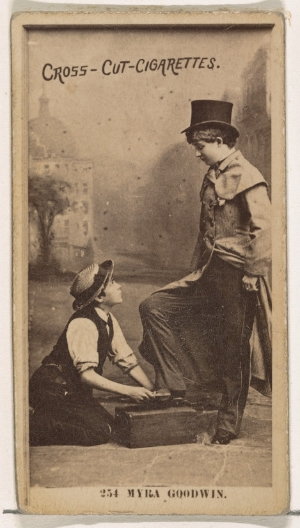
\includegraphics[width=0.5\textwidth]{images/1}
    \caption{A teapot}
    \label{fig:1}
\end{figure}
Furthermore 7,443 images are available for verification.
Both the training and verification image-sets have an corresponding csv-file where one row corresponds with one image.
The images are labeled using numbers, an additional csv-file is given containing the corresponding attributes for each number.
There are 1103 labels in total.
\begin{figure}[h]
    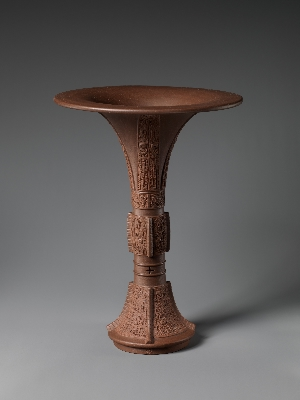
\includegraphics[width=.2\textwidth]{images/3}
    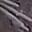
\includegraphics[width=.2\textwidth]{images/4}
    \caption{Example images from the dataset}
    \label{fig:2}
\end{figure}

\section{Scope}
We want to train a classifier that predicts labels for unknown images as good as possible.
To reach this goal, we will implement an convolutional neural network, then optimize its hyper-parameters.
\section{Implementation}
For implementation we plan to use Python 3.7 with keras\cite{KERAS} and sciPY\cite{SCIPY}, in particular numpy and pandas. 
As an extension of the project we look towards trying out different libraries, such as fast.ai\cite{FASTAI} and compare the different results.
% If we have enough time left at the end of the project we might also try different libraries and compare if we can get better results that way.


\bibliographystyle{plainnat}
\bibliography{bibliography}


\end{document}